\documentclass{report} %[twoside] ?
\usepackage[utf8]{inputenc}
\usepackage[english]{babel}
\usepackage{graphicx}
\usepackage{array}
\usepackage{amssymb, mathtools}
\usepackage{setspace}
\usepackage{multirow}
\usepackage{subcaption}
\usepackage{caption}
\usepackage{changepage}
\usepackage{xurl}
\usepackage{xcolor}
\usepackage{titlesec}
\usepackage{hyperref}
\captionsetup{font=footnotesize}
\titleformat{\chapter}[display]
    {\normalfont\huge\bfseries}{\chaptertitlename\ \thechapter}{20pt}{\Huge}
\titlespacing*{\chapter}{0pt}{0pt}{40pt}
\newcommand{\todo}[1]{\textcolor{red}{TODO: #1}}

\title{
    Title
}

\author{Julian Hendrik Freiherr Bock von Wülfingen}
\date{23.04.2025}

\begin{document}

\onehalfspacing

\pagenumbering{gobble}

\begin{titlepage}

	\begin{center}

        \vspace*{\baselineskip}

        {\Large Bielefeld University}
        
        \vspace{1.75\baselineskip}

        {\LARGE \scshape Title \\ of \\ Thesis\par} % Title

        \vspace{5\baselineskip}
        
        {\Large Julian Hendrik Freiherr Bock von Wülfingen}
        
        \vspace{2\baselineskip}

        {\Large Master Thesis\vspace{1em}}
        
        \textit{in Intelligent Systems \vspace{1em} \\ AG Machine Learning}
	
        \vfill

        \vspace{0.3\baselineskip}
        
        Primary Supervisor:     Michiel Straat\\
        Secondary Supervisor:   Pedro Fonseca\\
        Date:		            XX.XX.2025

    \end{center}

\end{titlepage}

\tableofcontents

\cleardoublepage
\pagenumbering{arabic}

\chapter*{Abstract}

\textbf{Objective}: In this work, we present an automatic detection model for Sleep-Disordered Breathing (SDB) events, particularly Sleep Apnea events. Sleep Apnea is a common sleep disorder affecting roughly 10\% of the population, and is associated with severe health risks. We aim to develop an easy and unobtrusive way of diagnosing SDB that helps with the large number of undiagnosed cases.

\noindent\textbf{Methods}: We trained an Attention U-Net architecture on PPG and optionally SpO2 signals from 1,880 overnight recordings of the MESA dataset to detect SDB events on a second-by-second basis. We evaluated the model performance using a strict event-level scoring method and compared the results to those of other studies. Another input to the model was the sleep stage information obtained from a pre-trained cardiorespiratory sleep staging model that used only PPG.

\noindent\textbf{Results}: We achieved a peak event-level detection F1-score of 69.7\% and a correlation of $\rho = 0.917$ for AHI prediction using PPG and SpO2. Reducing this setup to only use PPG, we achieved an F1-score of 61.6\% and a correlation of $\rho = 0.842$. We also showed the importance of using accurate sleep stage information, as providing the model with the ground-truth hypnogram increased the F1-score to 76.1\%, while not using any sleep stage information at all resulted in an F1-score of 56.9\%.

\noindent\textbf{Conclusion}: We present a state-of-the-art SDB detection model that uses only PPG and SpO2 signals, which are easy to set up and unobtrusive during sleep. We also show that using surrogate sleep stage information is a valid approach to improve performance, even if it is not as good as the ground-truth hypnogram. Our model can help with the large number of undiagnosed SDB cases and can be used for long-term monitoring of patients.

\chapter{Title for Intro \label{Chapter-Intro}}

\section{Section}

\subsection*{Subsection}

\chapter{Methods \label{Chapter-Methods}}

\section{Dataset}

\begin{itemize}
    \item Explain MESA (what Patients, how did they record the nights, ...)
    \item Statistical analysis (Count, Age, ...)
    \item Scorings from SOMNOLYZER (OSA, HYP, ...)
    \item Kappa between NSRR and SOMNOLYZER
    \item Use predicted Hypnogram (maybe?) and their Kappa
\end{itemize}

\section{Preprocessing}

\begin{itemize}
    \item PPG [256Hz], SpO2 [1Hz], Hypnogram [1Hz]
    \item For PPG: Statistical Analysis, Denoising, VAE?, Conv-Block
\end{itemize}

\section{Model Architecture}

\begin{itemize}
    \item U-Net (with PPG Conv-Block), Batch-Norm, Attention, ...
    \item Output: Detection at 1Hz - Event vs No Event
    \item TODO Next model then classifies into SDB classes
\end{itemize}

\section{Training and Evaluation}

\begin{itemize}
    \item Training Parameters (Optimizer, LR, BS, ...) and Setup (Machines, ...)
    \item Seed and Cross-Validation
    \item Train on 30min (?) segments. For Testing: Concat 30min Windows with Overlap for full night result.
    \item Correct results (like Olsen, 10sec minimum event and distance between events)
    \item Event-based metrics (Se, Pr, F1) and when to count TP, TN, FP, FN
    \item AHI-based metric (Linear Correlation, Severity Classes, Near-Boundary Double-Classification)
\end{itemize}

% \subsection*{Subsection}

\chapter{Results \label{Chapter-Results}}

\section{PPG Preprocessing through the VAE}

One of the preprocessing techniques used to "downsample" the PPG signal was the Variational Autoencoder (VAE), whose encoder could be used to transform each 256Hz second into a 1Hz value of 8 dimensions. We tried two versions: The first got a 1-second input and had to reconstruct the exact second. The other one go a 2-second window around the second it should reconstruct. Figure \ref{fig:vaereconstruction} shows the example reconstructions of the two variations and Figure \ref{fig:vaeloss} plots the reconstruction losses over the epochs. As the 5s VAE had a lower loss, we used its encoder for the VAE preprocessing option.

\begin{figure}[h]
    \centering
    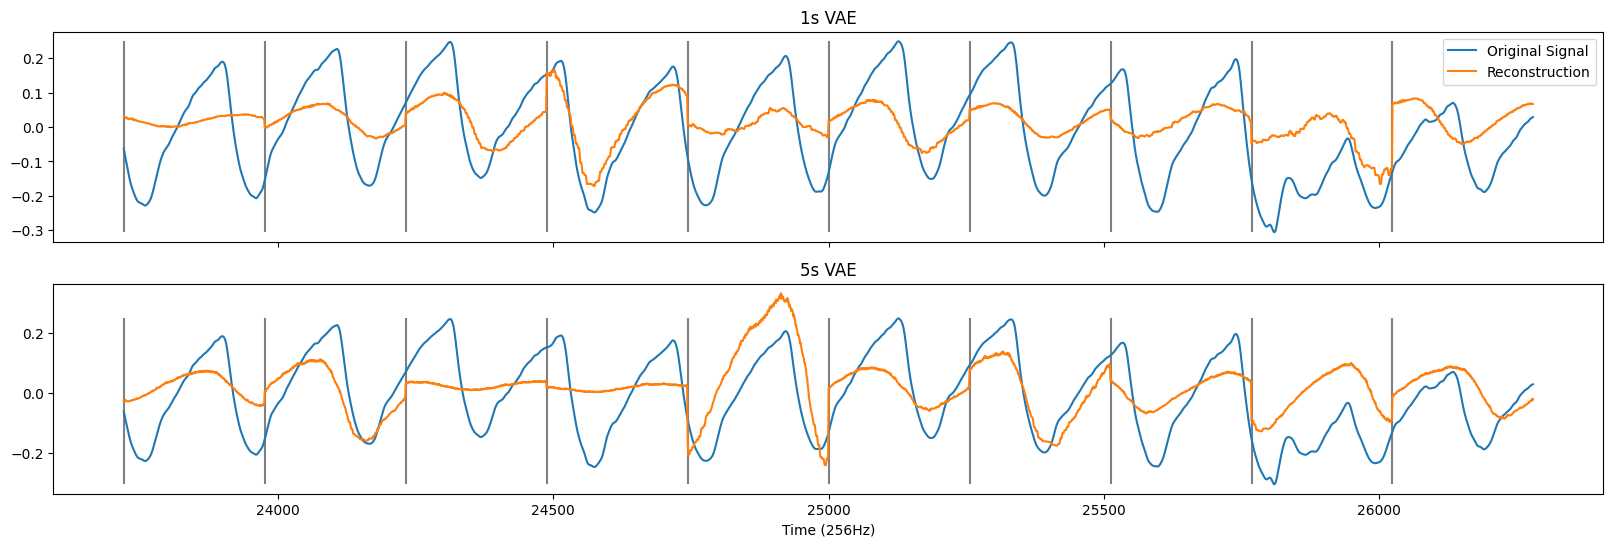
\includegraphics[width=\textwidth]{images/VaeReconstruction}
    \caption{Example difference in reconstructions of the 1s and 5s VAE for the same signal. Each second has 256 values, which are reduced to only 8 values.}
    \label{fig:vaereconstruction}
\end{figure}

\begin{figure}
    \centering
    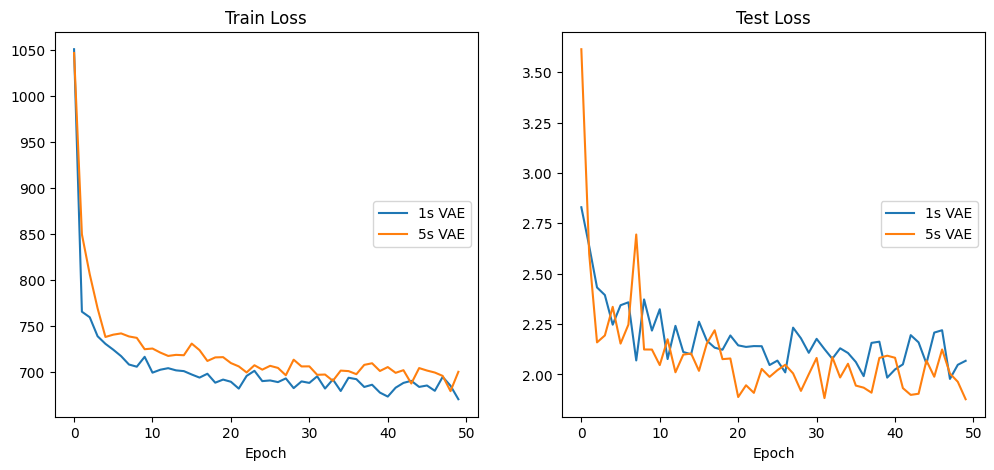
\includegraphics[width=\textwidth]{images/VaeLoss}
    \caption{Train and test loss of both VAEs. Although the 1s VAE had a lower train loss, the 5s performed better on the test set, which could be a sign of better generalization.}
    \label{fig:vaeloss}
\end{figure}

\section{Preprocessing impact on performance}

Figure \ref{fig:preprocessingresults} shows the recall, precision, and F1-score for the SDB detection model with the different preprocessing techniques. While neither the statistical nor the VAE preprocessing approach reached the same performance as the in-model approach, using both statistical and VAE preprocessing together did reach a similar performance. As both these values would only be needed to be calculated once before the training and not during each epoch, which the in-model approach did, training time got reduced significantly by a factor of 3. This can be seen in Table \ref{tab:preprocessing-times}.

\begin{figure}
    \centering
    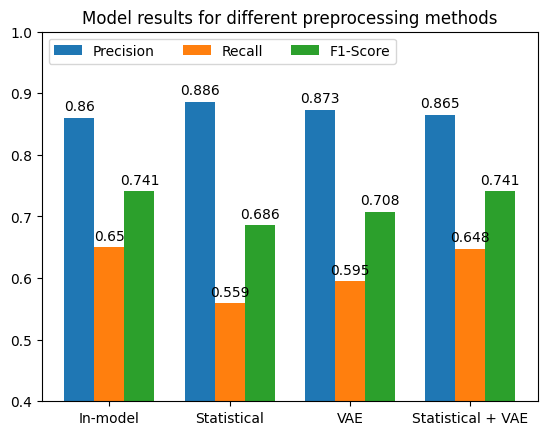
\includegraphics[width=0.6\textwidth]{images/PreprocessingResults}
    \caption{Precision, recall, and F1-score of the SDB detection model with different preprocessing techniques. Although the precision didn't change much, the recall and therefore the F1-score dropped significantly, when using the statistical or VAE preprocessing only.
    Important to note is that these results came from experiments with the ground-truth hypnogram, which is not the final model, as the final model uses the PPG-predicted hypnogram.}
    \label{fig:preprocessingresults}
\end{figure}

\renewcommand{\arraystretch}{1.5}
\begin{table}
    \centering
    \begin{tabular}{ l c c }
        Method & Training time & Testing time \\
        \hline
        In-model & 145min & 34min \\
        Statistical & 46min & 12min \\
        VAE & 47min & 12min \\
        Stat. + VAE & 50min & 12min \\
    \end{tabular}
    \caption{SDB detection model training and testing times in minutes. The in-model approach took roughly three times as long. \label{tab:preprocessing-times}}
\end{table}

\section{SDB Detection Model}

\subsection*{Event-level performance}

Figure \ref{fig:event-metrics} shows the recall, precision, and F1-score over each threshold for the main SDB detection model, which uses the PPG-predicted hypnogram, the PPG itself with the in-model technique, and the SpO2. The Figure also shows a version of the model without the SpO2 signal, which means it relies solely on the PPG data. As can be seen, omitting the SpO2 signal has a significant impact on the performance, as the peak F1-score drops from 69.7\% to 61.6\%.

\begin{figure}
    \centering
    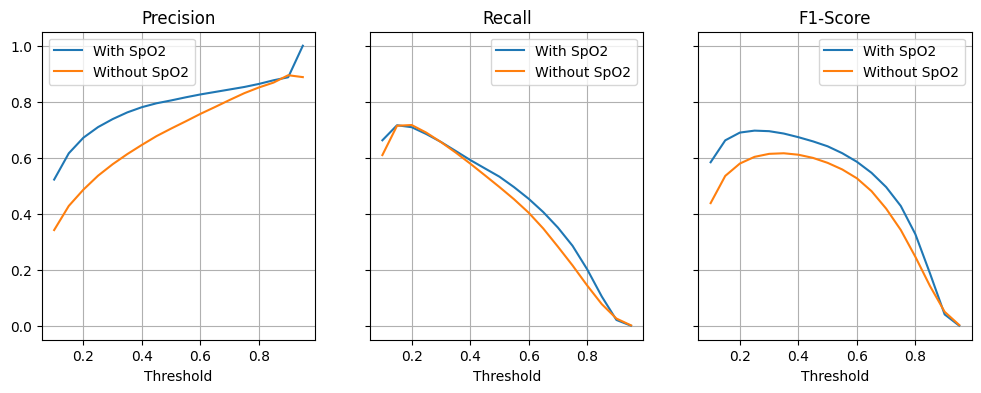
\includegraphics[width=\textwidth]{images/DetectionModelEventMetrics}
    \caption{Comparison of the event-level metrics of the SDB detection model with and without SpO2. The model with SpO2 reached a peak F1-score of 69.7\% at a threshold of 0.25, while the one without SpO2 only reached a peak F1-score of 61.6\% at a threshold of 0.35.}
    \label{fig:event-metrics}
\end{figure}

Test and training losses together with the peak F1-score over the epochs are displayed in Figure \ref{fig:event-epoch-losses}. While the version without SpO2 seems to train slightly more stable, learning convergences much slower than the one with SpO2, which reaches the area of the final peak F1-score in the first few epochs.

\begin{figure}
    \centering
    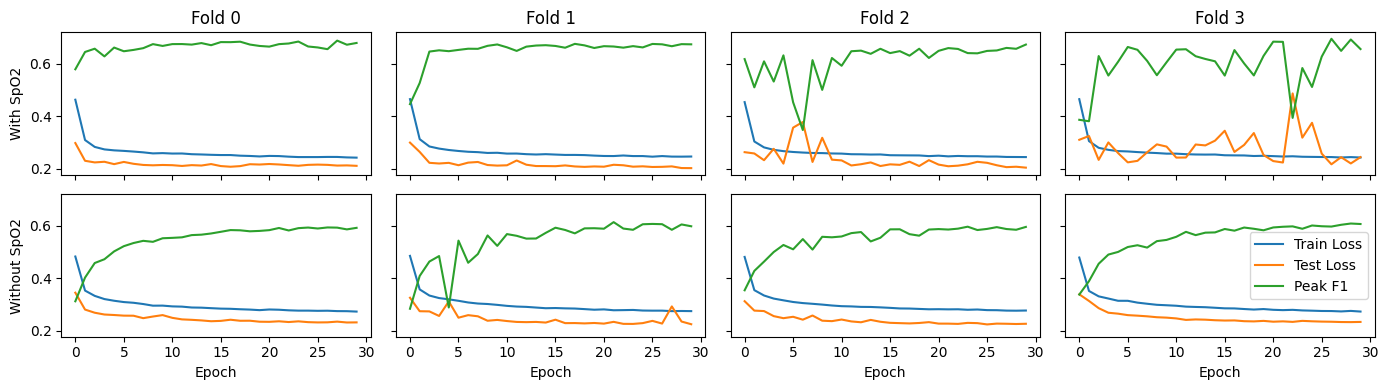
\includegraphics[width=\textwidth]{images/DetectionModelEpochLosses}
    \caption{Losses and peak F1-score by epoch for every fold.}
    \label{fig:event-epoch-losses}
\end{figure}

The threshold for the best performance was determined to be 0.25 and the final event-level metrics are shown in Table \ref{tab:final-metrics}.

\renewcommand{\arraystretch}{1.5}
\begin{table}
    \centering
    \begin{tabular}{ l c }
        Metric & Score \\
        \hline
        Precision & 70.94\% \\
        Recall    & 68.46\% \\
        F1-Score  & 69.68\% \\
    \end{tabular}
    \caption{Final metrics for the SDB detection model trained on the PPG-predicted hypnogram, the SpO2 signal, and the in-model processed PPG at a classification threshold of 0.25. \label{tab:final-metrics}}
\end{table}

With this threshold, we can analyse the performance based on the event class and sleep stage. Table \ref{tab:event-class-distribution} shows the distribution of event classes in the dataset and the models detection rate. The dataset is highly imbalanced, with 2/3 of all events being hypopneas. Still, the model was best in detecting mixed apneas, with a near 90\% detection rate, while hypopneas were only detected about 2/3 of the time.

\renewcommand{\arraystretch}{1.5}
\begin{table}
    \centering
    \begin{tabular}{ l p{2cm} p{2cm} p{2cm} p{2cm} }
        & Obstructive \newline Apnea & Mixed \newline Apnea & Central \newline Apnea & Hypopnea \\
        \hline
        Total (N) & 61161 & 4811 & 15240 & 162536 \\
        \% of all & 25.1\% & 2.0\% & 6.3\%  &  66.7\% \\
        \hline
        Found (N) & 43243 & 4299 & 12486 & 111826 \\
        \% found & 70.7\% & 89.4\% & 81.9\% & 68.8\% \\
    \end{tabular}
    \caption{Distribution of event classes in the full dataset and how many of the different classes were detected by our model. Although the dataset is greatly inbalanced to hypopneas (2/3 of all) and against mixed apneas (only 2\%), the detection rates greater for apneas than for hypopneas. \label{tab:event-class-distribution}}
\end{table}

In appendix \todo{ref} we show and discuss the results per sleep stage and the length of the predicted events.

\subsection*{AHI-level performance \todo{both this and the next section need to be reworked after the new AHI calculation}}

Figure \todo{ref} shows the scatter plots for the predicted and true AHI values of both versions of the model \todo{address the bias towards predicting lower AHIs}. To assess agreement, Figure \todo{ref} displays the corresponding Bland-Altman plots. We found a \todo{highlight the interesting metrics, like level of agreement, ICC, Spearman's rank, ...}. All AHI-level metrics can be found in Table \todo{ref}.

\subsection*{Severity-class-level performance}

Figure \todo{ref} shows the confusion matrices for the predicted severity classes using the hard thresholds and the NBL version. Although a strong focus on the true prediction diagonal can be seen, the bias towards predicting lower severity classes is also visible like in the AHI-level results.

We shows the models discrimination ability in Table \todo{ref}. \todo{which values to highlight?}

\section{Importance of correct Sleep Stages}

To assess the importance of the correct sleep stage prediction, we trained a model with the ground-truth hypnogram, the PPG-generated hypnogram, and finally without any sleep stage information, letting the model only rely on PPG and SpO2. Figure \ref{fig:sleep-stage-importance} shows the event-level metrics for each of these experiments. With the exception of the recall for lower thresholds, the models performance reduces consistently, the less certain it is on sleep stages. Peak F1-score for the model without a hypnogram was only 56.9\%, a 13\% drop from the version with the PPG-predicted hypnogram and a 20\% drop from the model that has access to the ground-truth sleep stages, which got up to 76.1\%.

\begin{figure}
    \centering
    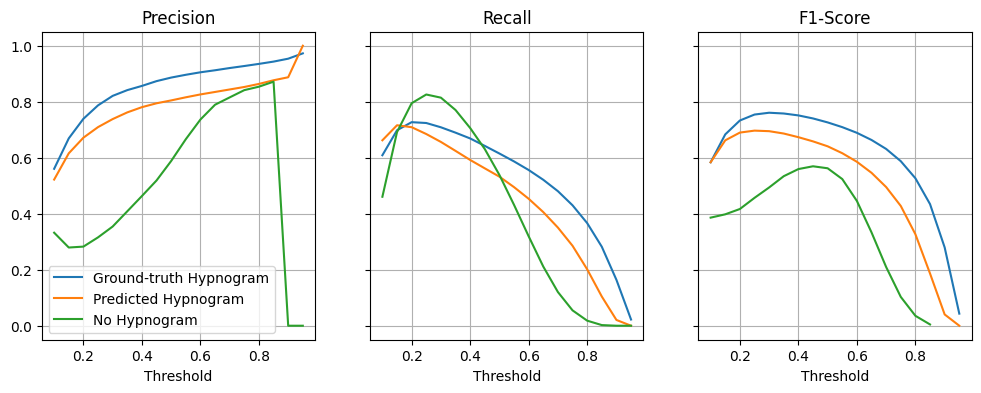
\includegraphics[width=\textwidth]{images/SleepStages}
    \caption{Precision, recall, and F1-score for the SDB detection model with different sleep stage information. The more the models sleep stage information gets to the ground-truth hypnogram, the better the performance.}
    \label{fig:sleep-stage-importance}
\end{figure}

\section{Correcting model output}

After applying the threshold for the prediction, a correction step was applied. This step removed events shorter than a specified number of seconds (called the correction size) and merged events that were closer than the correctification size. Figure \ref{fig:correction-size} displays the impact of the correctification size and shows that settings this value too low allows more prediction errors to pass through, while setting it too high removes many true positives. A correction size of 3 seconds seems to be the best option.

\begin{figure}
    \centering
    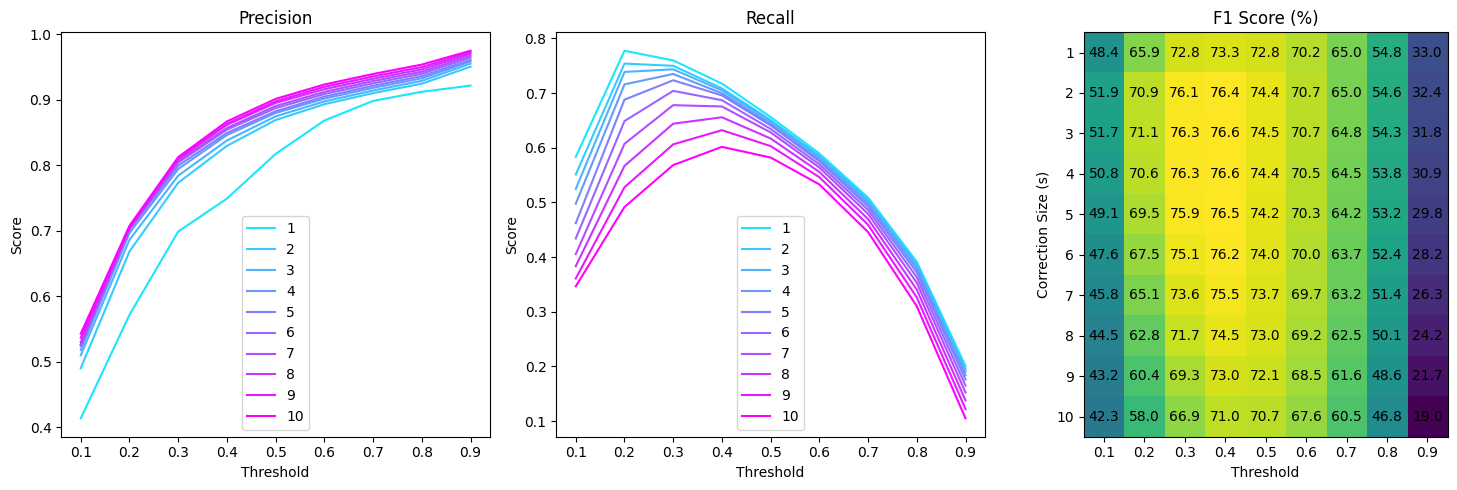
\includegraphics[width=\textwidth]{images/CorSizeMetrics}
    \caption{Event-level metrics for our SDB detection model for different correction sizes over the thresholds. As the precision grows with bigger correction sizes, the recall decreases. While most of both changes are somewhat evenly, there is a big difference in no correction (size of 1) to a small correction (of size 2) for the precision. Important to note is that, as with the preprocessing experiments, these results came from tests with the ground-truth hypnogram.}
    \label{fig:correction-size}
\end{figure}


\chapter{Discussion \label{Chapter-Discussion}}

% Discussions

In this work, we presented a, automatic, data-driven SDB detection model based on an Attention U-Net with state-of-the-art performance, that can tackle the problem of the huge number of undiagnosed sleep apnea cases, due to its selection of uncomplicated and inobtrusive input sensors. We achieved a peak F1-score of 76.6\% in event detection and an AHI prediction correlation of ???, which could be even further improved through the use of linear of MLP-based corrections. We showed great diagnostic results with positive and negative likelihood ratios of $\ge 16$ and $\le 0.28$ respectively with very few participants being wrongly classified more than one severity class apart. All metrics were based on our strict event scoring that is more transparent than minute-to-minute, segment classification.

Our model demonstrated higher detection rates for apnea events compared to hypopnea events. This result, while counterintuitive given the event distribution in the dataset, is expected because hypopneas are harder to detect due to their lower impact and not always being associated with desaturation events.

One goal of our work was to use only PPG and SpO2, as the finger-worn sensor recording these signals, is easy to set up and unobtrusive during sleep. However, an even less obtrusive option are smart watches or smart rings, that already today can record PPG at good quality. To our knowlegde, SpO2 cannot be realiably be recorded using these devices, especially not the subtle drops in saturation on which some classification is based on. 
We showed that omitting SpO2 data from the training signals decreased performance, but not as much as expected. The model was still able to detect SDB events with a peak F1-score of \todo{X\%} and predict AHI with a correlation of \todo{X}. This means that our model is still usefull on these unobtrusive technologies that only measure PPG, and can be used over many nights. This greatly helps with diagnositic meaningfulness, screening, analyzing night-to-night variability, and evaluating effectiveness of SDB treatment methods.
Also, \todo{appendix XY} showed that training without SpO2 data was, while plateauing way slower, more stable than than training with it, which is likely due to the fact that SpO2 in itself is less stable and prone to artifacts. 

Another important factor of our models performance is the use of sleep stage labels. The model performed best when using ground truth sleep stages from Somnolyzer and worst without any sleep stage information. The PPG-derived sleep stages from \cite{bakker2021estimating} greatly improved results over using no sleep stage information but were still not as good as using the ground truth. Further improvements in predicting the hypnogram from only PPG signals could lead to better results in detecting SDB, that are still relying solely on data from PPG sensors.

We also looked into preprocessing the PPG signal using statistical analysis and a VAE. While achieving the same level of perfomance as using the in-model approach, training time of the detection model decreased significantly. Inference time will not be affected, as the benefit comes only from not needing to recompute the preprocessed signal for each training run, but this approach could help with rapid prototyping and hyperparameter tuning.

Finally, correcting the models output by filtering out events shorter than 3 seconds and merging events less than 3 seconds apart into one, we saw an increase in event-level results, while general AHI-level performance decreased slightly. Looking at the positive and negative diagnostic performance, we see that correcting the output improves results on high AHI participants while slightly lowering results on low AHI participants. This explains lower general AHI-level performance, as the dataset is slightly biased towards low AHIs.

% Limitations

An important limitation of our work is the lack of validation on other datasets. While the MESA dataset we used is large and greatly balanced in some regards, like AHI, BMI, smoking habits, or co-morbidities, other factors like age are not balanced. Recordings have also been made in a clinical setting and with the same hardware. Even further, first-night effects haven't been adressed.
Validation our work on other datasets, is crucial to show generalizability and usefulness of our model in the real world.

% Future work

Future work could tackle the bias and errors in AHI prediction. While a linear correctioin could help correcting the bias, other studies have shown that using demographic data to refine the AHI through a small MLP can increase correlation greatly.

As the use of smart watches or smart rings maximizes or goal of inobtrusive SDB detection even further, future work could also look into using other sensors that are already available on these devices. One example is the accelerometer, which records movements during sleep, or breathing sounds, that are mainly used for detecting snoring. Both signals are indicators of SDB events and might improve our results even further.

\chapter{Conclusion \label{Chapter-Conclusion}}

In this work we aimed to create an easy to set up and unobtrusive way to diagnose SDB, an illness that, while having significant health implications, is often undiagnosed. We have shown that using only signals from a finger-worn PPG sensor, we can detect SDB with high accuracy. While our method is not perfect and performance of the gold standard PSG is still not reached, we believe that our method is a step in the right direction, helping with screening and pre-diagnosis of SDB.
\todo{ with state-of-the-art performance, that can tackle the problem of the huge number of undiagnosed sleep apnea cases, due to its selection of uncomplicated and inobtrusive input sensors.}
\todo{summery: importance of correct sleep stage}

\bibliographystyle{unsrt}
\bibliography{References.bib}

\appendix

\chapter{Appendix \label{Chapter-Appendix}}

\section{Predicted Sleep Stages\label{Apx-Pred-Hypnogram}}

To obtain sleep stage predictions for our model, we used a pre-trained cardiorespiratory sleep staging model, as described by Bakker et al. \cite{bakker2021estimating}. The model was designed to use any arbitrary combination of input signals to predict the 4-class hypnogram (Wake, combined N1/N2, N3, and REM). We opted to use only the PPG signal to fit our goal. When evaluating against Somnolyzer scorings of the MESA dataset, we achieved a Cohen's Kappa of 0.57, showing moderate agreement. Table \ref{tab:predicted-hypnogram-results} shows additional metrics and classification tasks, like a binary wake versus sleep task.

The performance is lower than reported in the original paper, which is due to the fact that they used additional input signals. Combining cardiac information with airflow, their algorithm reached a Kappa of 0.643 in 4-class classification and 0.680 when also incorporating respiratory effort.

\renewcommand{\arraystretch}{1.5}
\begin{table}[h!]
    \centering
    \makebox[\textwidth][c]{\begin{tabular}{ p{2.5cm} p{2cm} p{2.3cm} p{2.3cm} p{1.5cm} p{2.3cm} }
        Task & Kappa & Acc. & Se. & Sp. & PPV \\
        \hline
        4-cl. \newline (Wake/N1-\newline N2/N3/REM) & 0.566 \newline [0.436, 0.677] & 73.2\%\newline [64.8\%, 80.0\%] & - & - & - \\
        3-cl. \newline (Wake/NREM\newline/REM) & 0.628 \newline [0.473, 0.740] & 79.4\%\newline [70.8\%, 85.6\%] & - & - & - \\
        2-cl. \newline (Wake/Sleep) & 0.653 \newline [0.475, 0.778] & 84.6\% \newline [76.2\%, 90.3\%] & 73.1\% \newline [56.9\%, 84.9\%] & 91.8\% \newline (8.37\%) & 89.6\% \newline [79.0\%, 95.2\%] \\
    \end{tabular}}
    \caption{PPG-based sleep stage prediction performances against Somnolyzer scorings on different tasks. Values are presented as median and 25th and 75th percentiles, median [Q1, Q2], or (in case of normally distributed data) as mean and standard deviation, mean (sd). \label{tab:predicted-hypnogram-results}}
\end{table}

Figure \ref{fig:tst-plot} shows the true TSTs from Somnolyzer plotted against the predicted TSTs and the Bland-Altman-Plot. The sleep stage predictor achieved an RMSE of 1.1 (hours) and a Spearman rank correlation of 0.712.

\begin{figure}
    \centering
    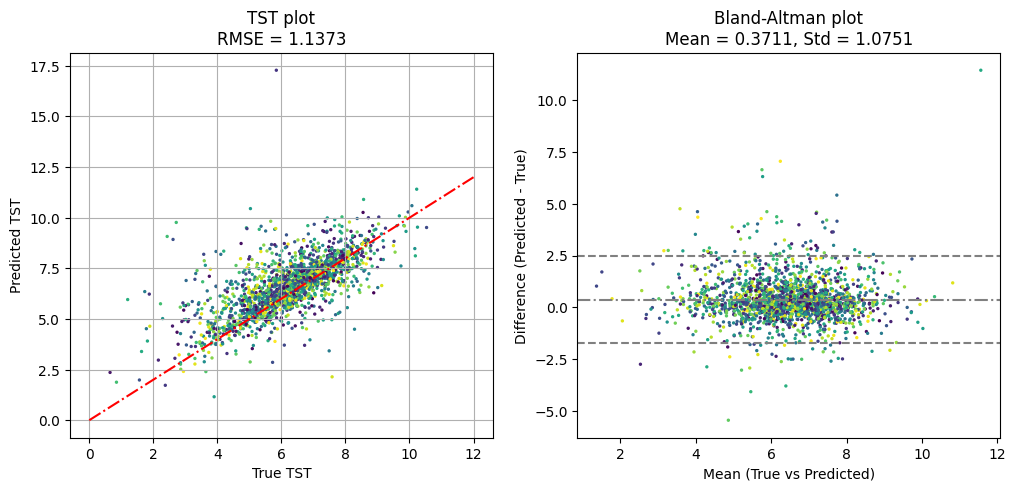
\includegraphics[width=\textwidth]{images/TstPlot}
    \caption{Predicted TST plotted against the true TST from Somnolyzer (left) and the Bland-Altman-Plot (right). The red line is the identity line. The upper and lower gray lines show the levels of agreement.}
    \label{fig:tst-plot}
\end{figure}

\section{Lowpass Denoising of the PPG Signal\label{Apx-Denoise}}

\begin{figure}[h!]
    \centering
    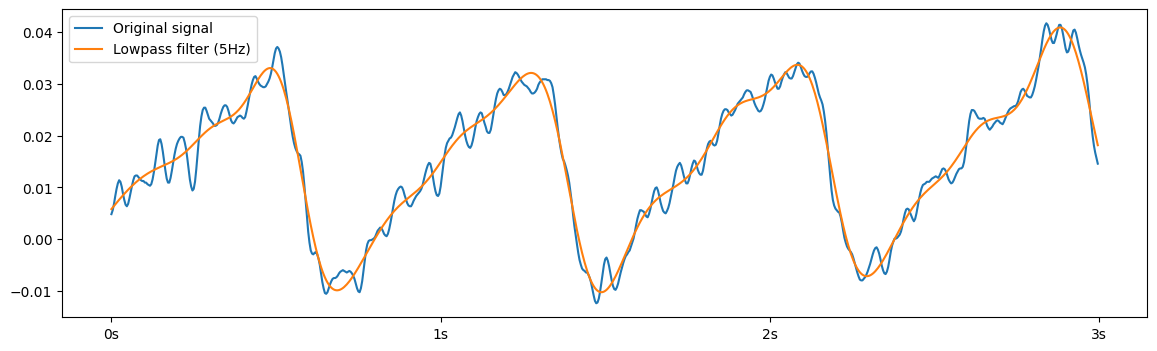
\includegraphics[width=\textwidth]{images/Lowpass}
    \caption{Comparison of the original signal (blue) and the denoised signal (orange) for a random 3-second PPG window from our dataset. We used a lowpass filter with a cutoff frequency of 5Hz.}
    \label{fig:lowpass-example}
\end{figure}

\section{Near-boundary Double-labeling\label{Apx-NBL}}

In NBL, single AHIs can get assigned to a second severity class, if they are near the boundaries. The specific values are as follows:

\renewcommand{\arraystretch}{1.5}
\begin{table}[h!]
    \centering
    \begin{tabular}{ l c c }
        Severity class & Hard boundaries & NBL boundaries \\
        \hline
        Normal   & $ AHI < 5 $         & $ AHI < 7 $             \\
        Mild     & $ 5 \le AHI < 15 $  & $ 2.4 \le AHI < 17.4 $  \\
        Moderate & $ 15 \le AHI < 30 $ & $ 12.4 \le AHI < 35.2 $ \\
        Severe   & $ 30 \le AHI $      & $ 26.6 \le AHI $        \\
    \end{tabular}
\end{table}

\section{Severity-class-level Metrics\label{Apx-Severity-Metrics}}

\renewcommand{\arraystretch}{1.5}
\begin{table}[h!]
    \centering
    \begin{tabular}{p{3cm} p{3cm} p{4cm}}
        Metric & Calculation & Meaning \\
        \hline
        Accurracy \newline (Acc) & $\frac{TP+TN}{TP+FP+FN+TN}$ & What \% got \newline correctly classified? \\
        Sensitivity \newline (Se, alt. Recall) & $\frac{TP}{TP+FN}$ & What \% of positives \newline got correctly \newline classified? \\
        Specificity \newline (Sp) & $\frac{TN}{TN+FP}$ & What \% of negatives \newline got correctly \newline classified? \\
        Positive Predicted \newline Value (PPV) & $\frac{TP}{TP+FP}$ & What \% of predicted \newline positives where \newline really positive? \\
        Negative Predicted \newline Value (NPV) & $\frac{TN}{TN+FN}$ & What \% of predicted \newline negatives where \newline really negative? \\
    \end{tabular}
\end{table}

\newpage
\section{Example Model Output\label{Apx-Output}}

\begin{figure}[h!]
    \centering
    \makebox[\textwidth][c]{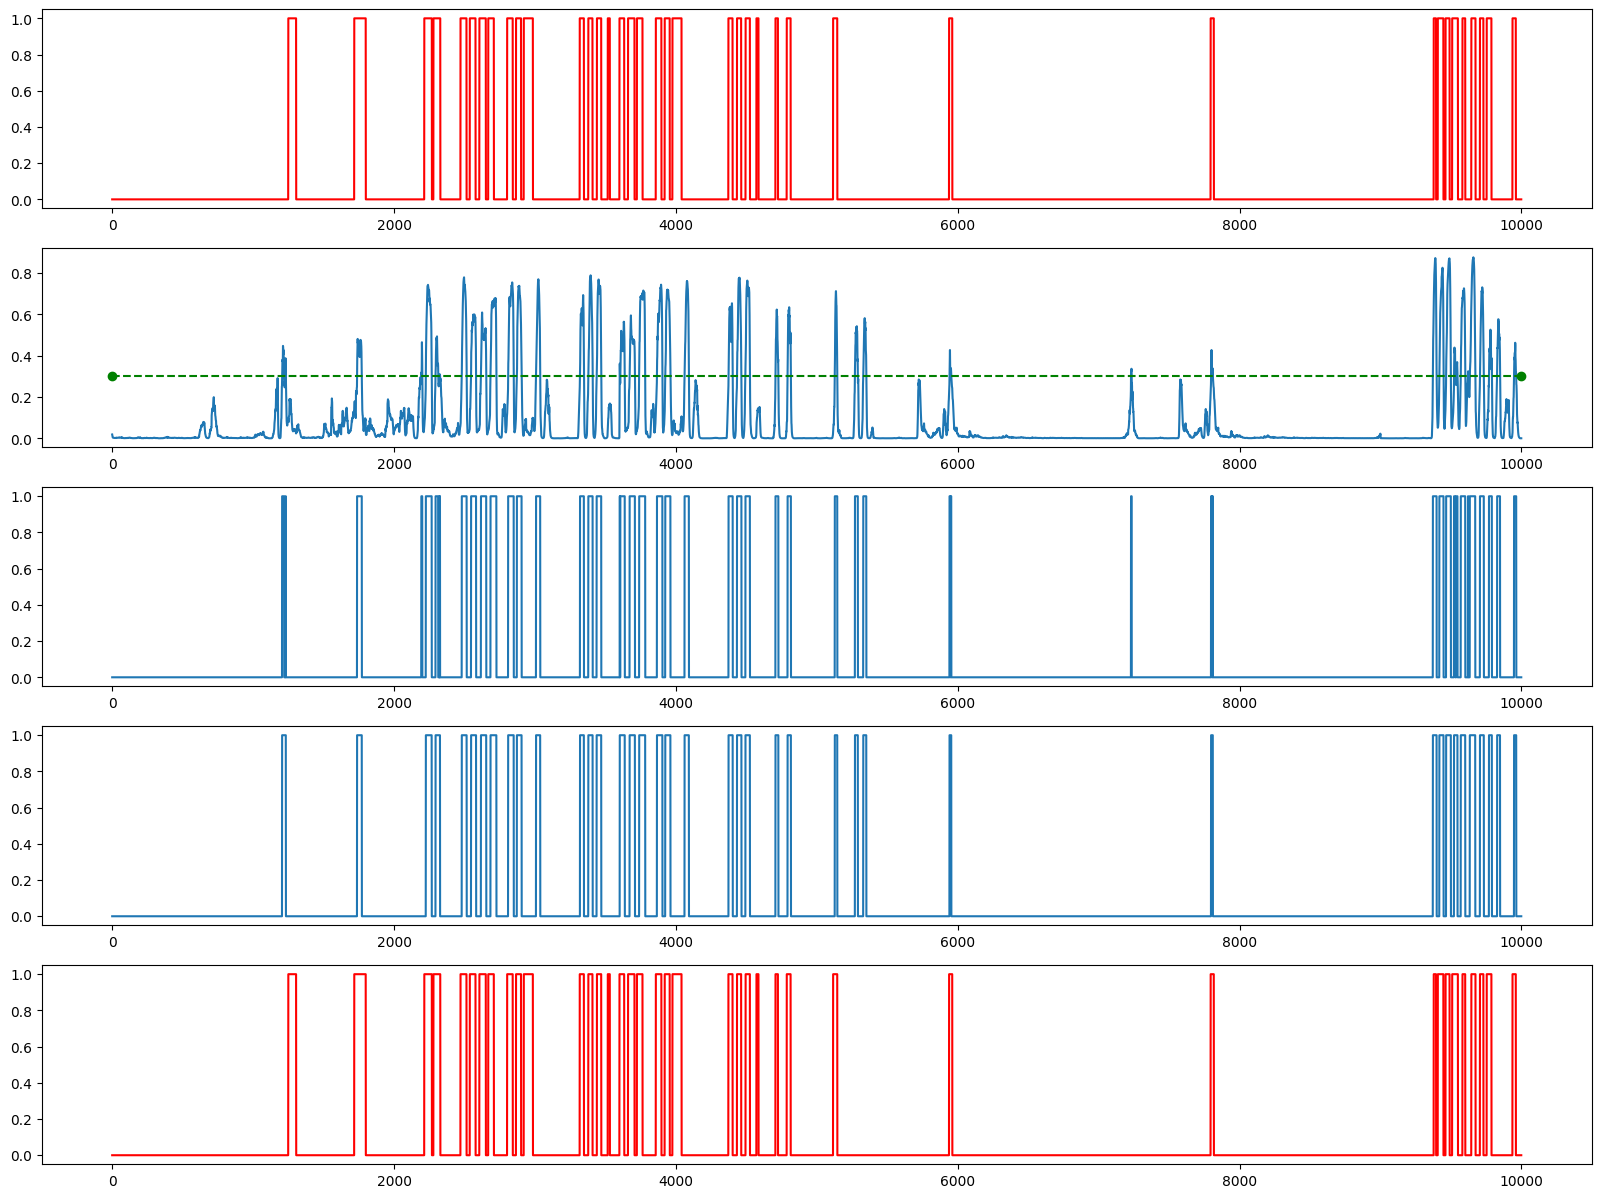
\includegraphics[width=1.2\textwidth]{images/ModelOutput}}
    \caption{Example of the model outputs: Top and bottom rows (red) show the true labels (event or not); the second row (blue) shows the predicted probabilities of the model's sigmoid layer; the third row (blue) shows an applied example threshold of 0.3; the fourth row (blue) shows the thresholded predictions after the correction step. One can see, how the correction step merges close events (e.g. the first event from the left) and removes too short events (e.g. the event around the second 7300).}
    \label{fig:example-output}
\end{figure}

\end{document}